% Poster Template for the Okinawa Institute of Science and Technology (OIST)
% Created by Jeremie Gillet on June 2019

\documentclass[
    a0paper, % Size of poster
    portrait, % Orientation
    fontscale=0.28 % General scaling for fonts, increase the number for smaller fonts (considered removing text first)
    ]{baposter}

% Graphics
\usepackage{graphicx} % Required for including images
\graphicspath{{figures/}} % Directory in which figures are stored

% Add any packages you need here
\usepackage{amsmath} % For typesetting math
\usepackage{caption}
\captionsetup{
  font=footnotesize,% set font size to footnotesize
  labelfont=bf % bold label (e.g., Figure 3.2) font
}
\newcommand{\beq}{\begin{equation}}
\newcommand{\eeq}{\end{equation}}
\newcommand{\beqs}{\begin{equation*}}
\newcommand{\eeqs}{\end{equation*}}
\newcommand{\of}[1]{\left(#1\right)}


% Defining colors
\selectcolormodel{HTML}
\definecolor{OIST}{HTML}{C80019} 
\definecolor{DarkRed}{RGB}{100,0,10}

% Changing fonts family
\renewcommand{\familydefault}{\sfdefault}
\usepackage{helvet}

% set the background of the poster
\background{
    \begin{tikzpicture}
        [remember picture,overlay]\node[opacity=1.0,below right] at (current page.north west) {
\includegraphics[width=1\paperwidth]{header_shisha}};
    \end{tikzpicture}
}

% Starting document, feel free to change the style of headers and boxes
% Documentation can be found here: http://www.brian-amberg.de/uni/poster/
% Unfortunately it is not very complete
\begin{document}
\begin{poster}{ % General poster options
    columns=4, % Number of columns, maximum 6
    eyecatcher=true, % Set to false for ignoring the left logo in the title and move the title left
    background=user, % Custom background
    linewidth=1.25pt, % Width of the border lines around content boxes
    textborder=rectangle, % Format of the border around content boxes, can be: none, bars, coils, triangles, rectangle, rounded, roundedsmall, roundedright or faded
    borderColor=OIST, % Border color
    headerheight=0.15 \textheight, % Height of the header
    headershape=rectangle, % Specify the rounded corner in the content box headers, can be: rectangle, small-rounded, roundedright, roundedleft or rounded
    headerfont=\large \sf \bf, % Large, bold and sans serif font in the headers of content boxes
    headerborder=closed, % Adds a border around the header of content boxes
    headershade=plain, % Single color in the background
    headerColorOne=white, % Background color for the header in the content boxes
    headerFontColor=DarkRed, % Text color for the header text in the content boxes
    boxColorOne=white, % Background color of the content boxes
} 
{} % No logo on the left
% Poster title
{\color{OIST}\Huge
 \textbf{Modeling Camphor Boat Speed \\ at the Air-Water Interface}
}
{ \vspace{1em} 
  Alexandru Mihai, Mahesh M. Bandi\\[0.5em]
  \small
  Collective Interactions Unit \\
  Okinawa Institute of Science and Technology Graduate University, Japan
  \vspace{3em} 
}

\begin{posterbox}[name=intro,column=0,span=4, row=0]{Introduction}
A camphor "boat" is propelled by the Marangoni force due to the ability of camphor to produce a surface tension gradient at the air-water interface. Its instantaneous speed at varying times throughout the life of the camphor boat reveals three distinct modes of motility; high speed motion with harmonic fluctuations, constant speed with small insignificant perturbations, and lastly relaxation oscillations characterized by long periods of little to no motion with sharp peaks in speed. Our model yields equilibrium points in the parameter space of the ODE system consistent with the experimental data. 
\end{posterbox}

%%%%%%%%%%%%%%%%%%%%%%%%%%%%%%

\begin{posterbox}[name=data1,column=0,span=2, below=intro]{Experimental Results}
In a glass petri dish filled with distilled water we introduce a circular camphor boat 3mm in diameter with 1mm thickness.
\begin{center}
\vspace{-2mm}
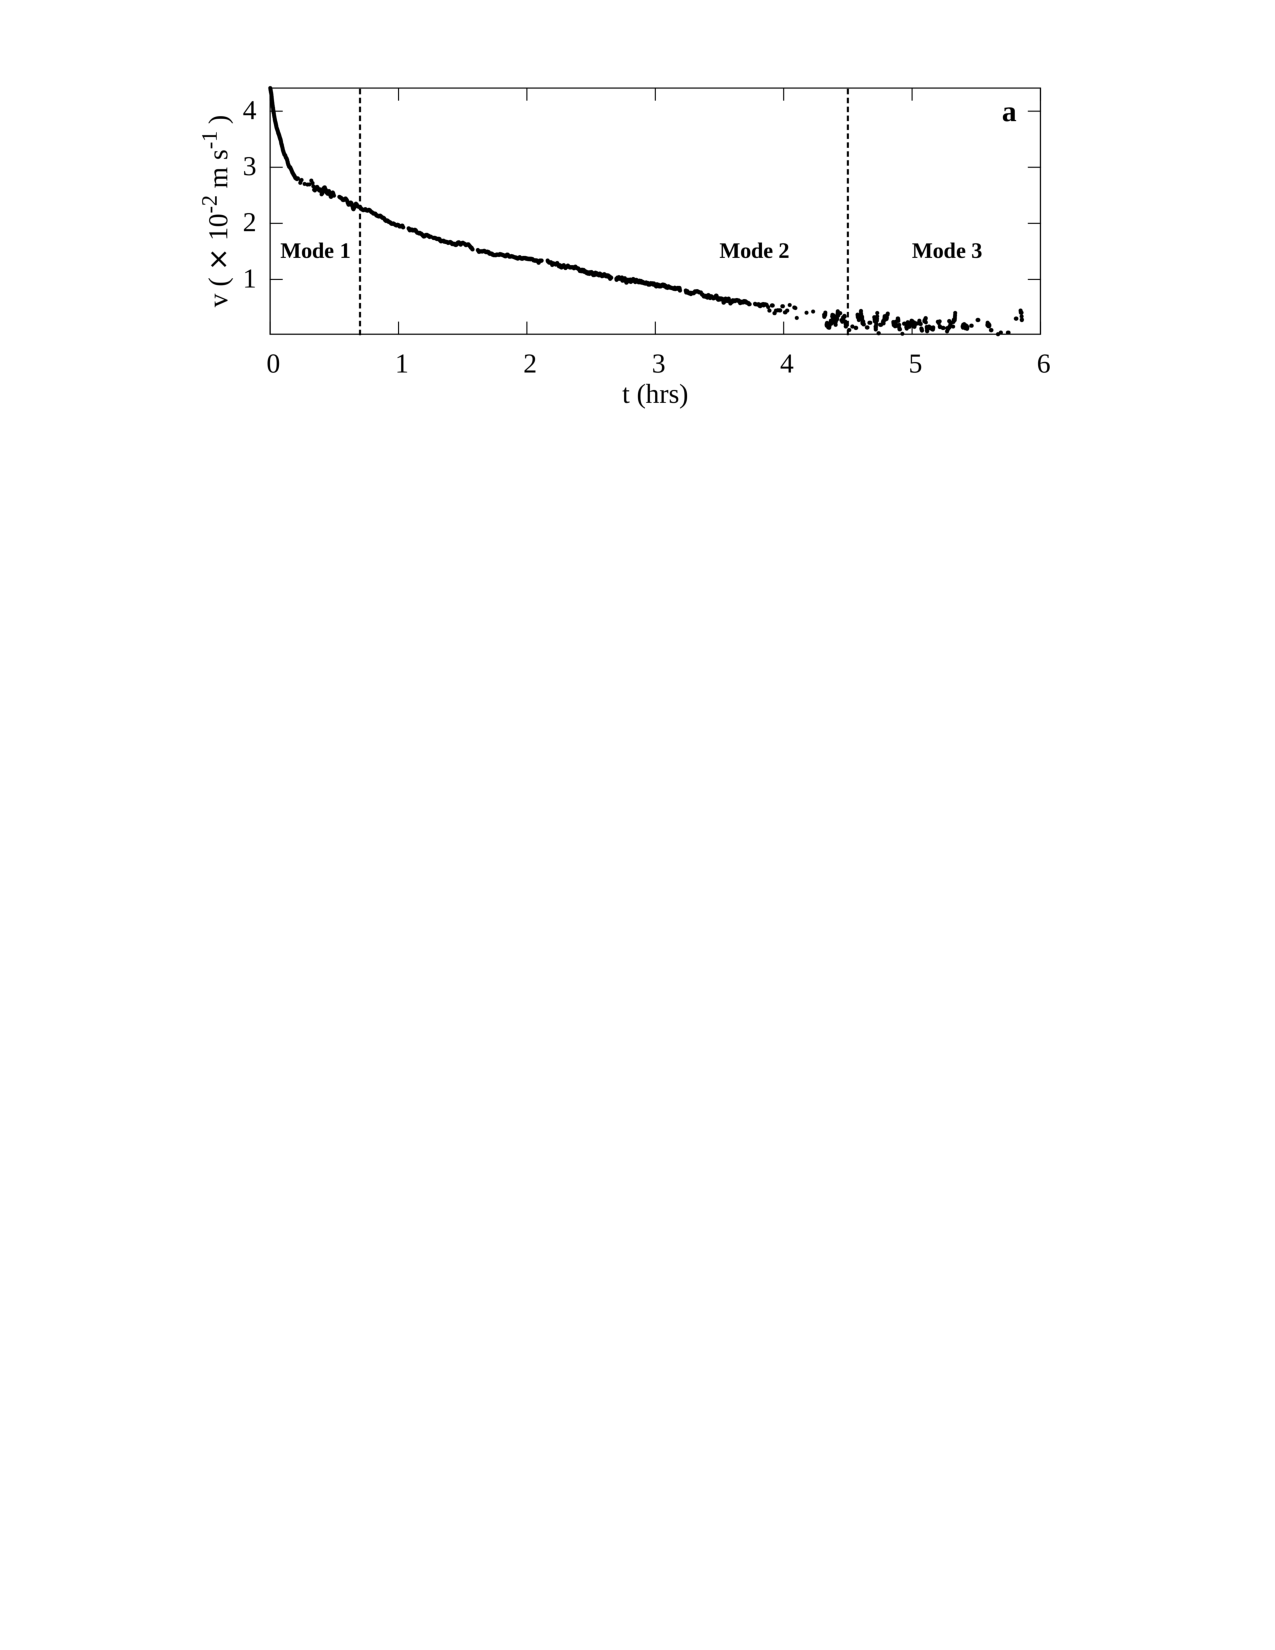
\includegraphics[width=\linewidth]{boat_speed_crop}
\vspace{-4mm}
\captionof{figure}{Average speed of a camphor boat at the air-water interface until consistent motion is no longer seen. Modes 1-3 refer to the local fluctuations in speed which correspond to varying dynamics in the system.}
\end{center}
\end{posterbox}

%%%%%%%%%%%%%%%%%%%%%%%%%%%%%%

\begin{posterbox}[name=camphor,column=0,span=2, below=data1]{Model of Camphor Depletion}

\setlength{\abovedisplayskip}{4pt}
\setlength{\belowdisplayskip}{4pt}

From Fig. 1 we infer that the concentration of camphor in the boat decreases exponentially. For given fitting parameters $\alpha$ and $\kappa$ we integrate this concentration and set it equal to a constant $\kappa$:
\beq\int_{t}^{t+\Delta t} e^{-\alpha t} \mathrm{d}t = \frac{1}{\alpha}\left[ e^{-\alpha t} - e^{-\alpha\of{t+\Delta t}}\right] = \kappa\eeq
we find an expression for the time it takes $\kappa$ amount of camphor to leech onto the surface:  
\vspace{-2mm}
\beq \Delta t  = -\frac{1}{\alpha}\ln\of{1-\alpha \kappa\cdot e^{\alpha t}} \eeq
Defining a recursive series based on the above equation starting at $t=0$ yields:
\vspace{-1mm}
\beq \Delta t_{n+1} =  -\frac{1}{\alpha}\ln\of{1-\alpha \kappa \cdot \exp\of{\alpha\displaystyle\sum_{i=0}^{n}\Delta t_i}} \label{delta_t}\eeq
The sequence $\Delta t_n$ gives the times at which the Marangoni force can act on the boat. To match the experimental data we set $\alpha=0.65$ and $\kappa=0.00015$.
\end{posterbox}

%%%%%%%%%%%%%%%%%%%%%%%%%%%%%%

\begin{posterbox}[name=data2,column=2,span=2, below=intro]{Camphor Boat Dynamics}


Narrowing the time averaging period of Fig. 1, three distinct dynamics are seen
\begin{center}
\vspace{-2mm}
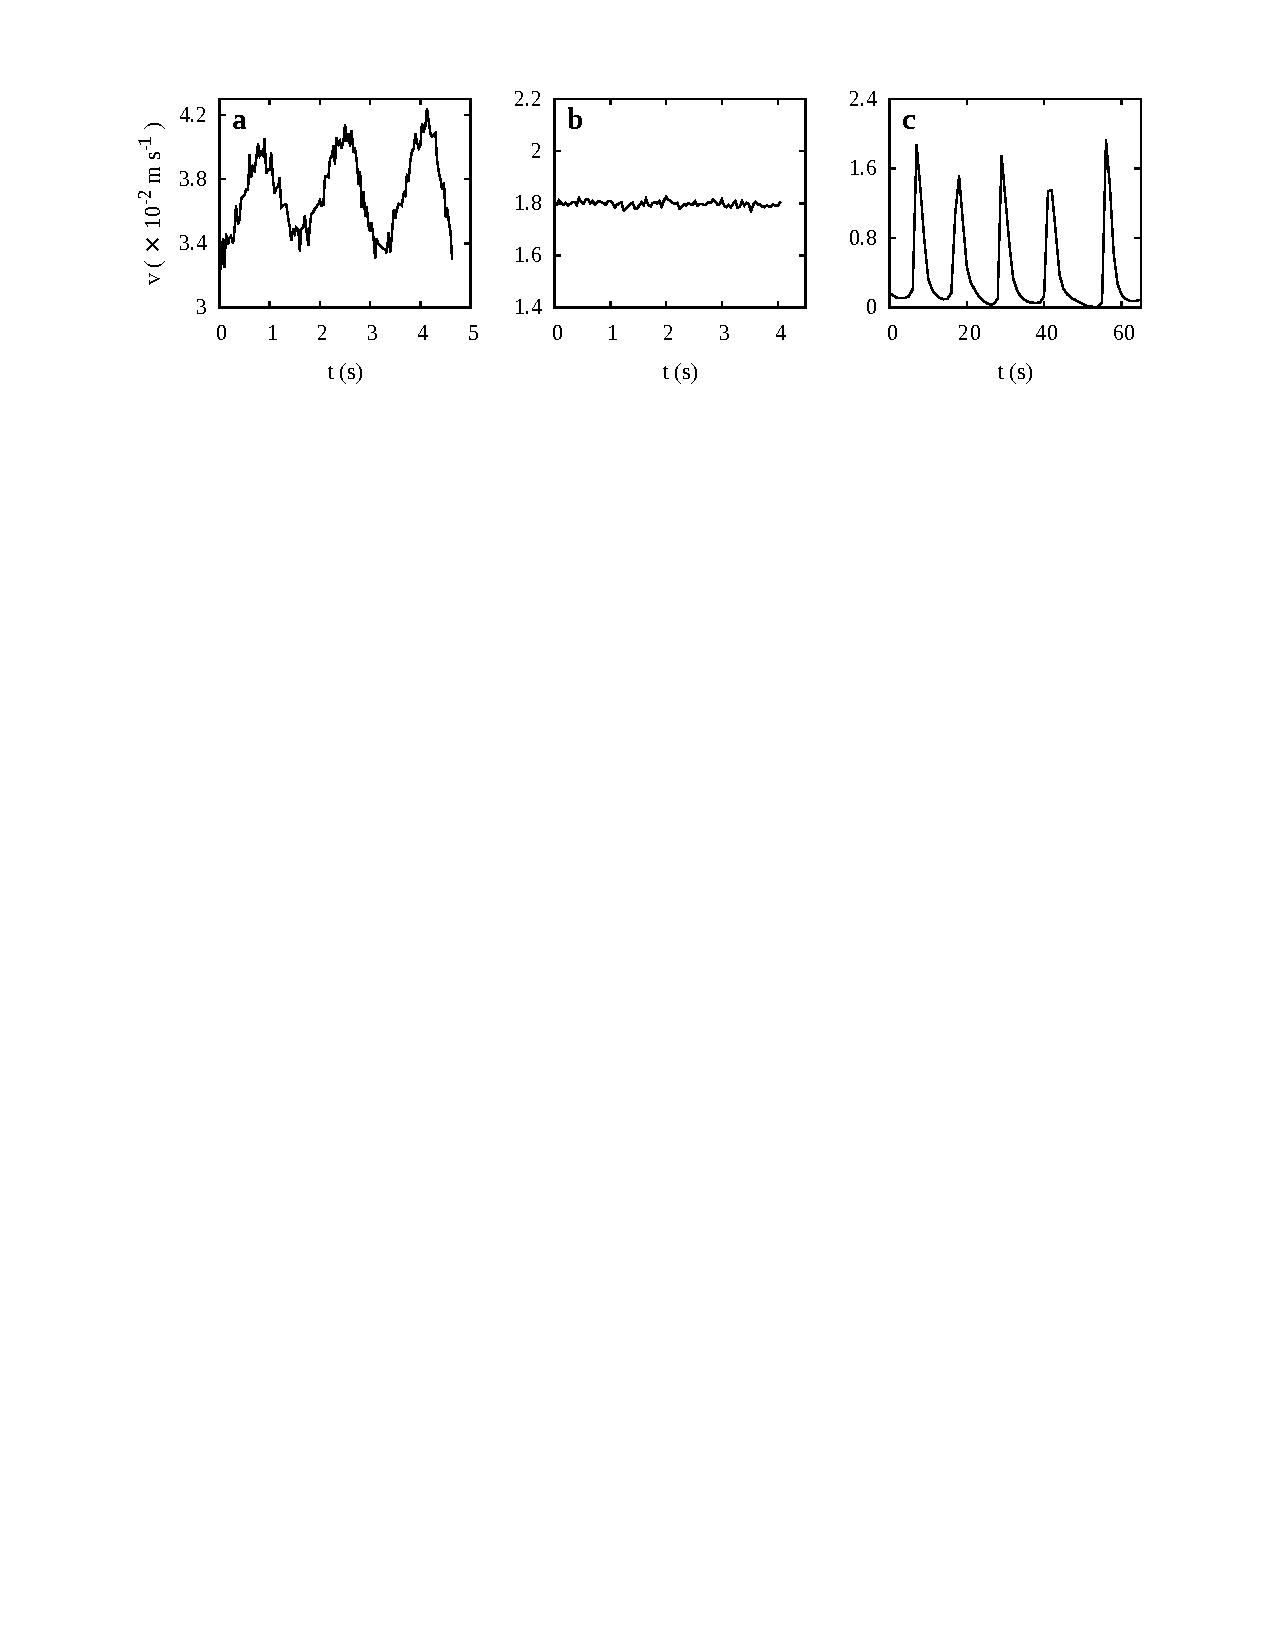
\includegraphics[width=\linewidth]{modes1-3}
\vspace{-5mm}
	\captionof{figure}{The instantaneous speed of the camphor boat shows the distinction between Modes 1-3 labeled in Fig. 1: ({\bf a}) harmonic oscillations of speed, ({\bf b}) a stable local speed, and ({\bf c}) relaxation oscillations in speed.}
\end{center}


\end{posterbox}

%%%%%%%%%%%%%%%%%%%%%%%%%%%%%%

\begin{posterbox}[name=van_der_pol,column=2,span=2, below=data2, bottomaligned=camphor]{Resulting Model of Camphor Speed}
A logical starting point is a system of ordinary differential equations encompassing harmonic oscillations as well as relaxation oscillations.
\vspace{-1mm}
\beq
\begin{aligned}
&  \frac{\mathrm{d}\nu}{\mathrm{d}\mathrm{t}} &=& \gamma\of{1-\chi^2}\nu-\chi&\\
&  \frac{\mathrm{d}\chi}{\mathrm{d}\mathrm{t}} &=& \nu&
\end{aligned}
\eeq\\[-3mm]
For $\gamma=0$ we see that the above system simplifies to a standard harmonic oscillator, and for large $\gamma>1$ we find relaxation oscillations, corresponding to Mode 1 and 3 in Fig. 1, respectively. To enable the model to exhibit the steady state solution of Mode 2 we make the following modifications:
\vspace{-2mm}
\begin{equation}
\begin{aligned}
\dot{\nu} = & \gamma\of{\of{\gamma-1}-\chi^2}\nu - \chi \\
\dot{\chi} = & \nu\frac{\of{1-\gamma}^2}{\gamma +1}
\end{aligned} 
\hspace{4mm}\hbox{given}\hspace{4mm}
\begin{aligned}
&\gamma = \frac{\Delta t_n}{0.007}&
\end{aligned}
\label{mine}
\end{equation}\\[-2mm]
Using the sequence $\Delta t_n$ from Eq. 3 we define $\gamma$ as above, where 0.007 is the characteristic time of relaxation oscillations found in Mode 3. 
\end{posterbox}


%%%%%%%%%%%%%%%%%%%%%%%%%%%%%%

\begin{posterbox}[name=simulation,column=0,span=4, below=camphor]{Simulation Results for $\gamma=\Delta t_n/0.007$}
\begin{center}
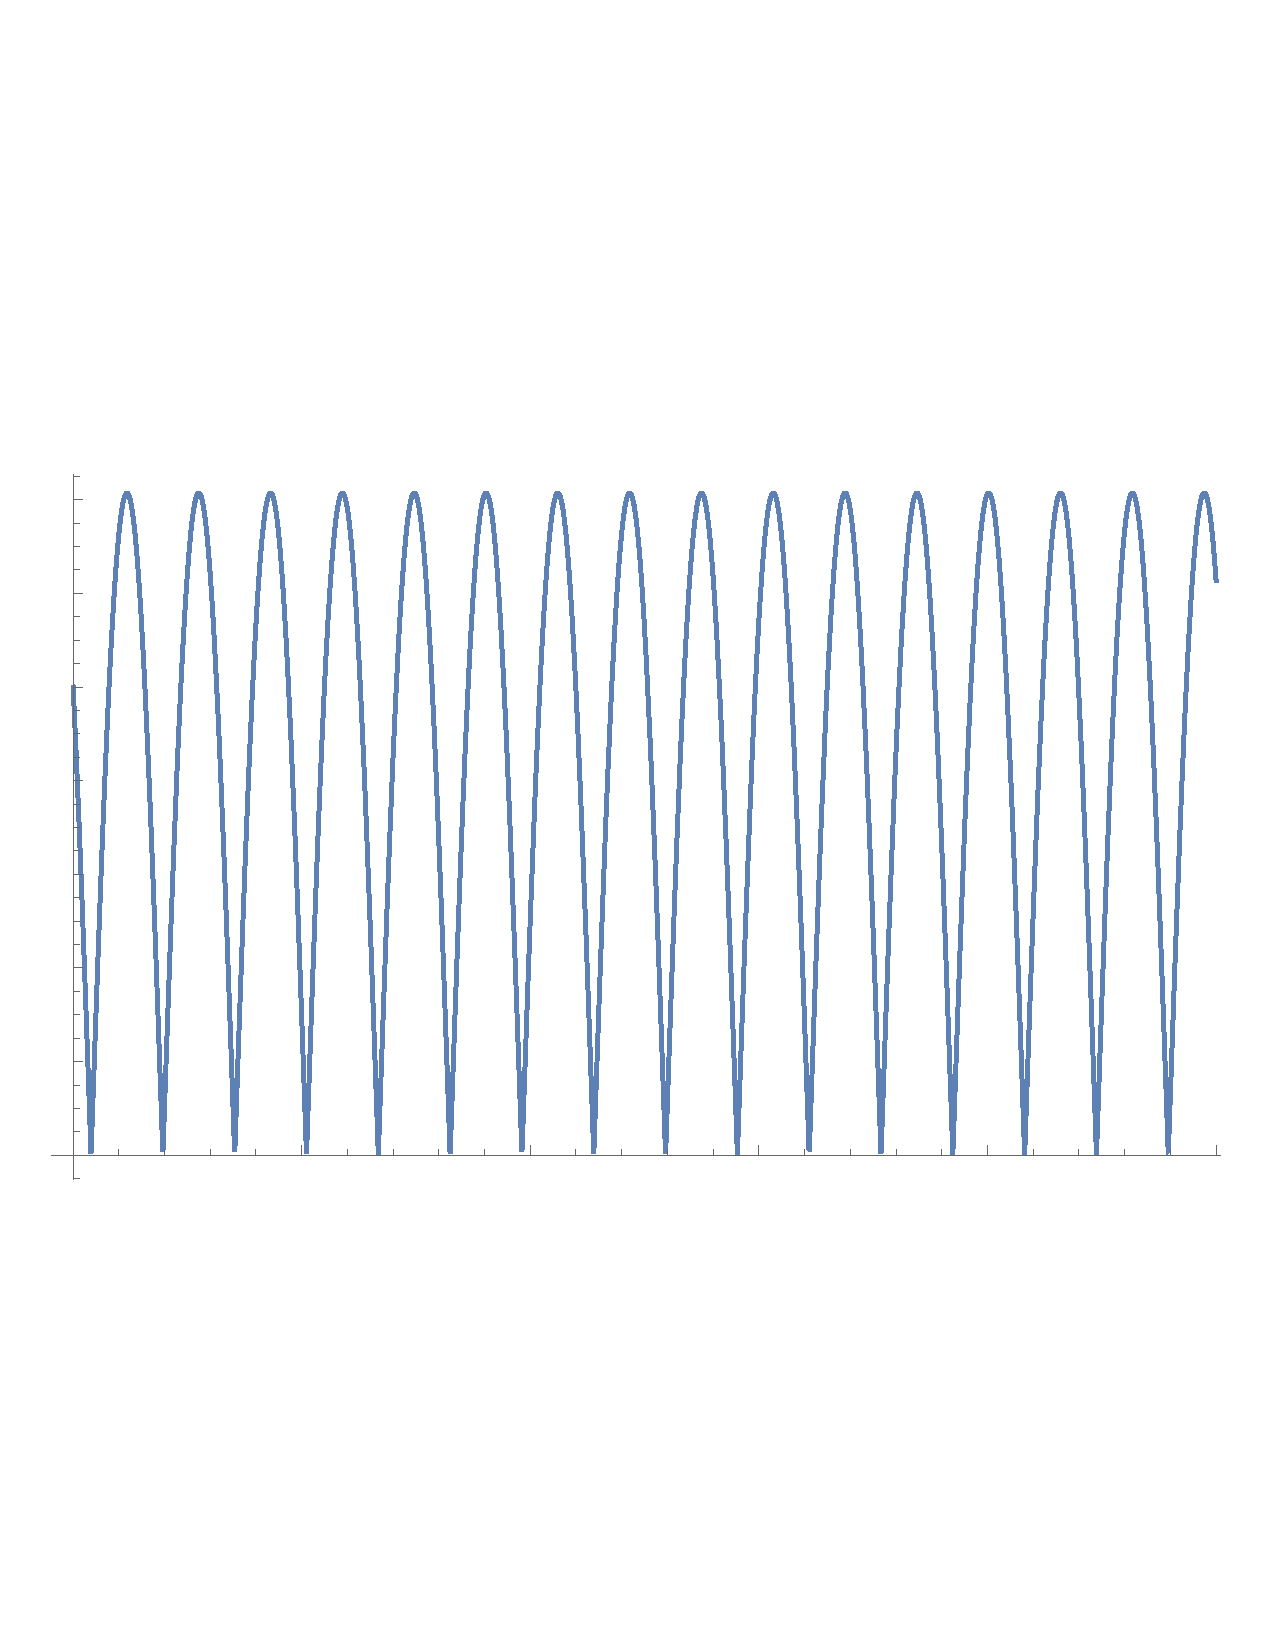
\includegraphics[width=.225\linewidth]{eq0_s.pdf}\hspace{3mm}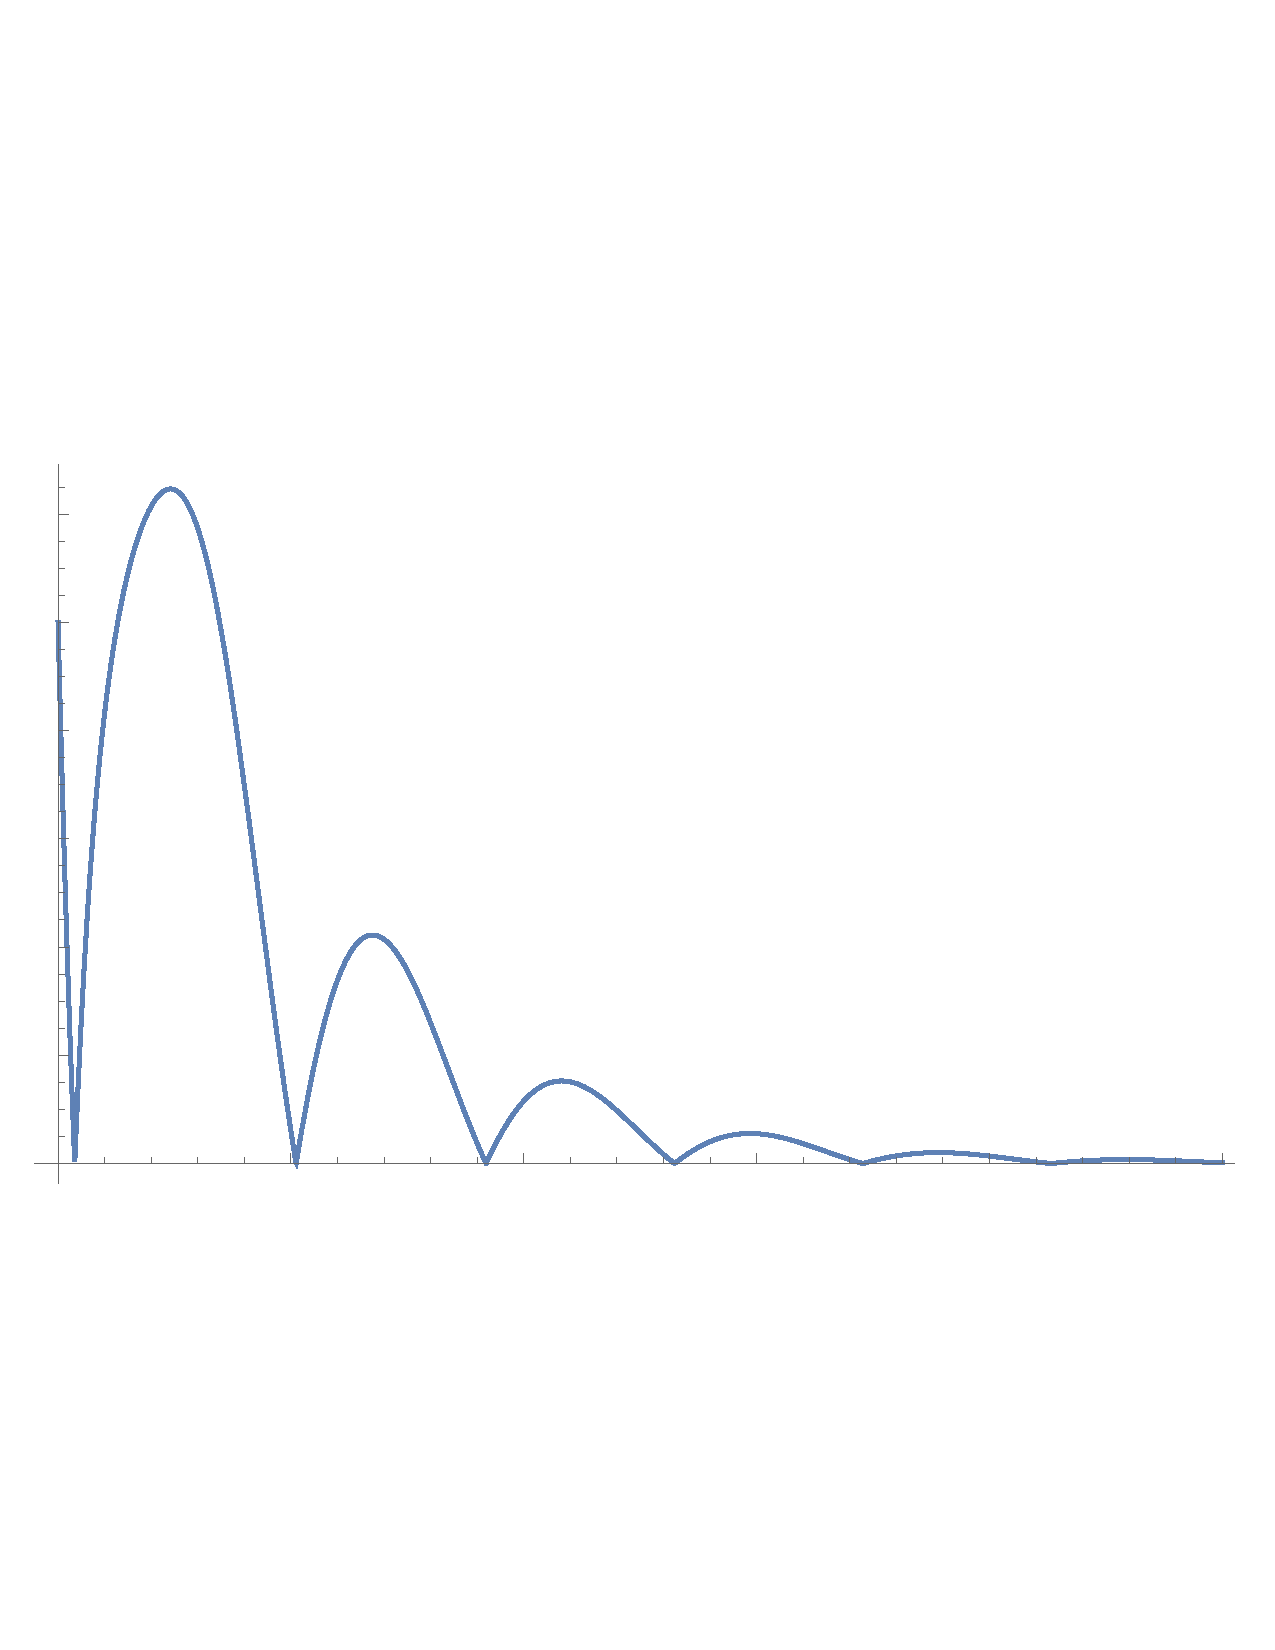
\includegraphics[width=.225\linewidth]{eq05_s.pdf}\hspace{3mm}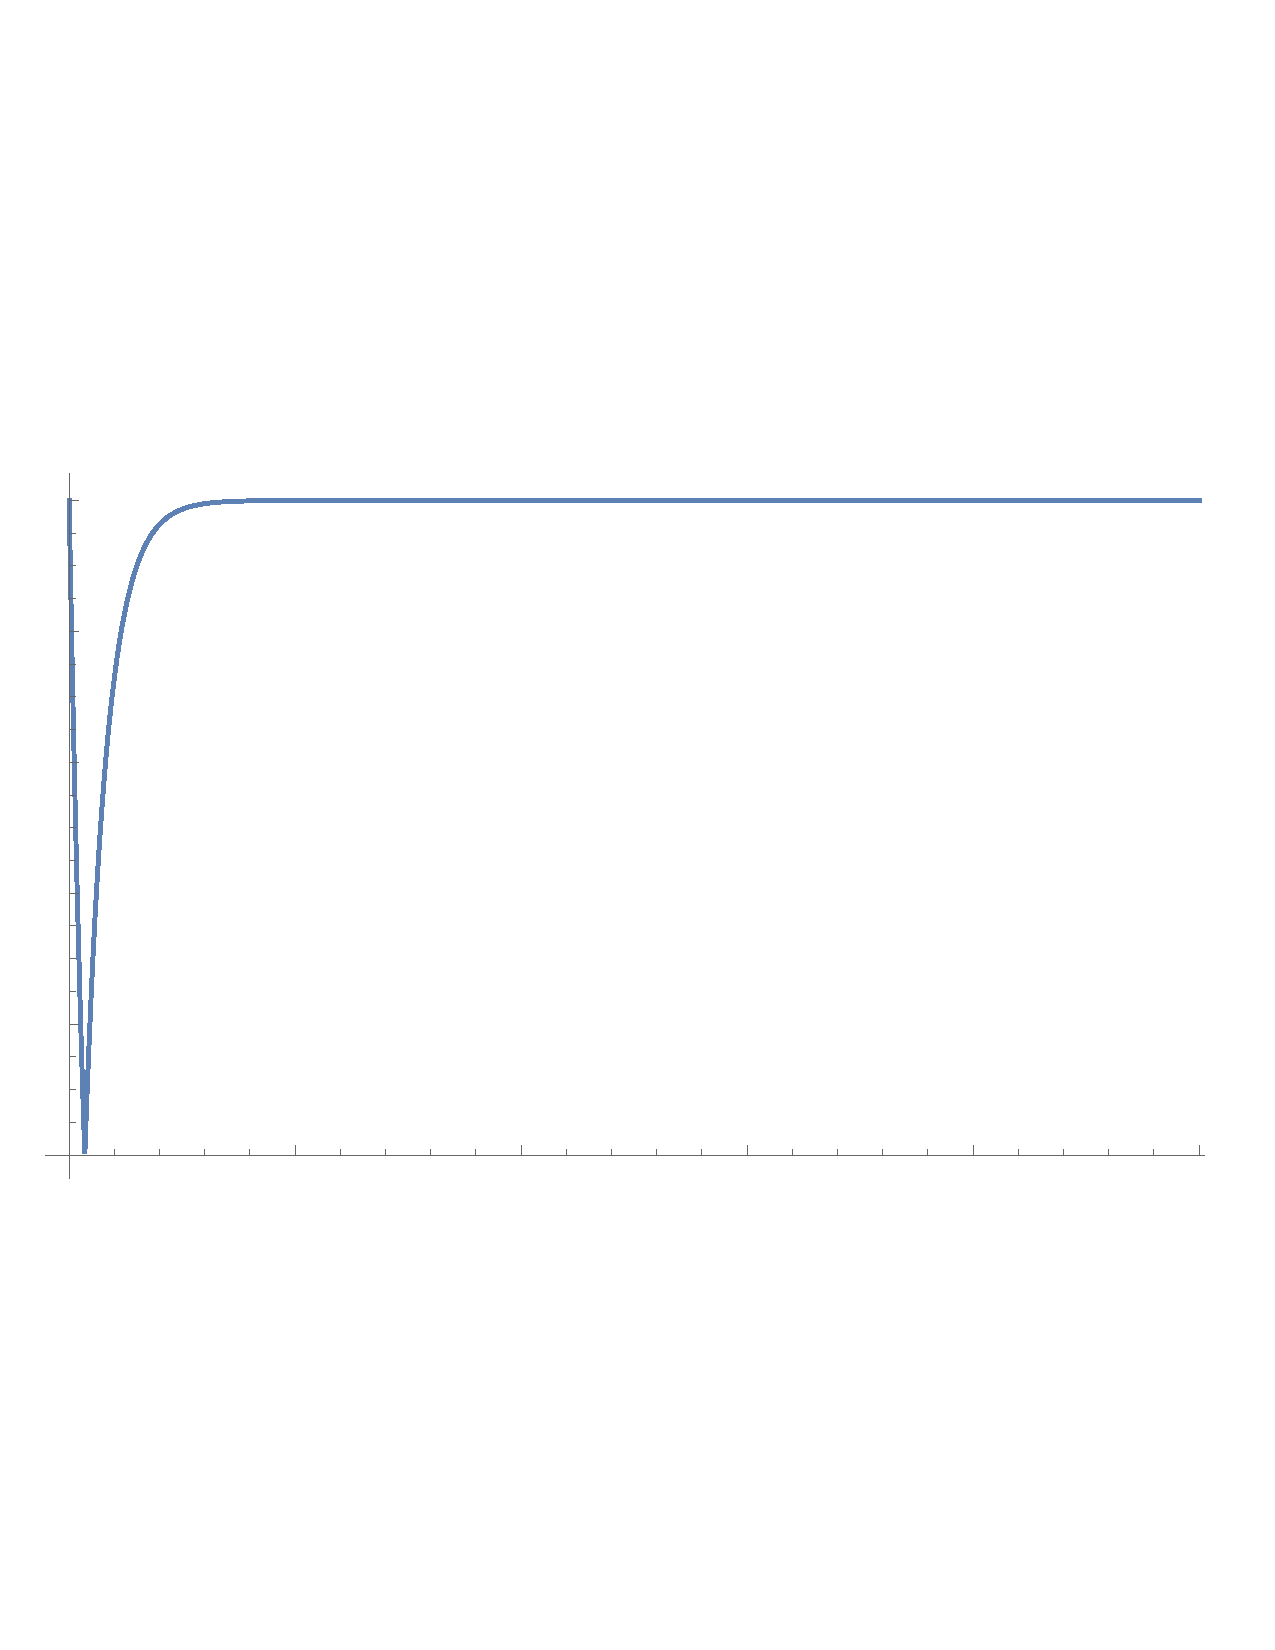
\includegraphics[width=.225\linewidth]{eq1_s.pdf}\hspace{3mm}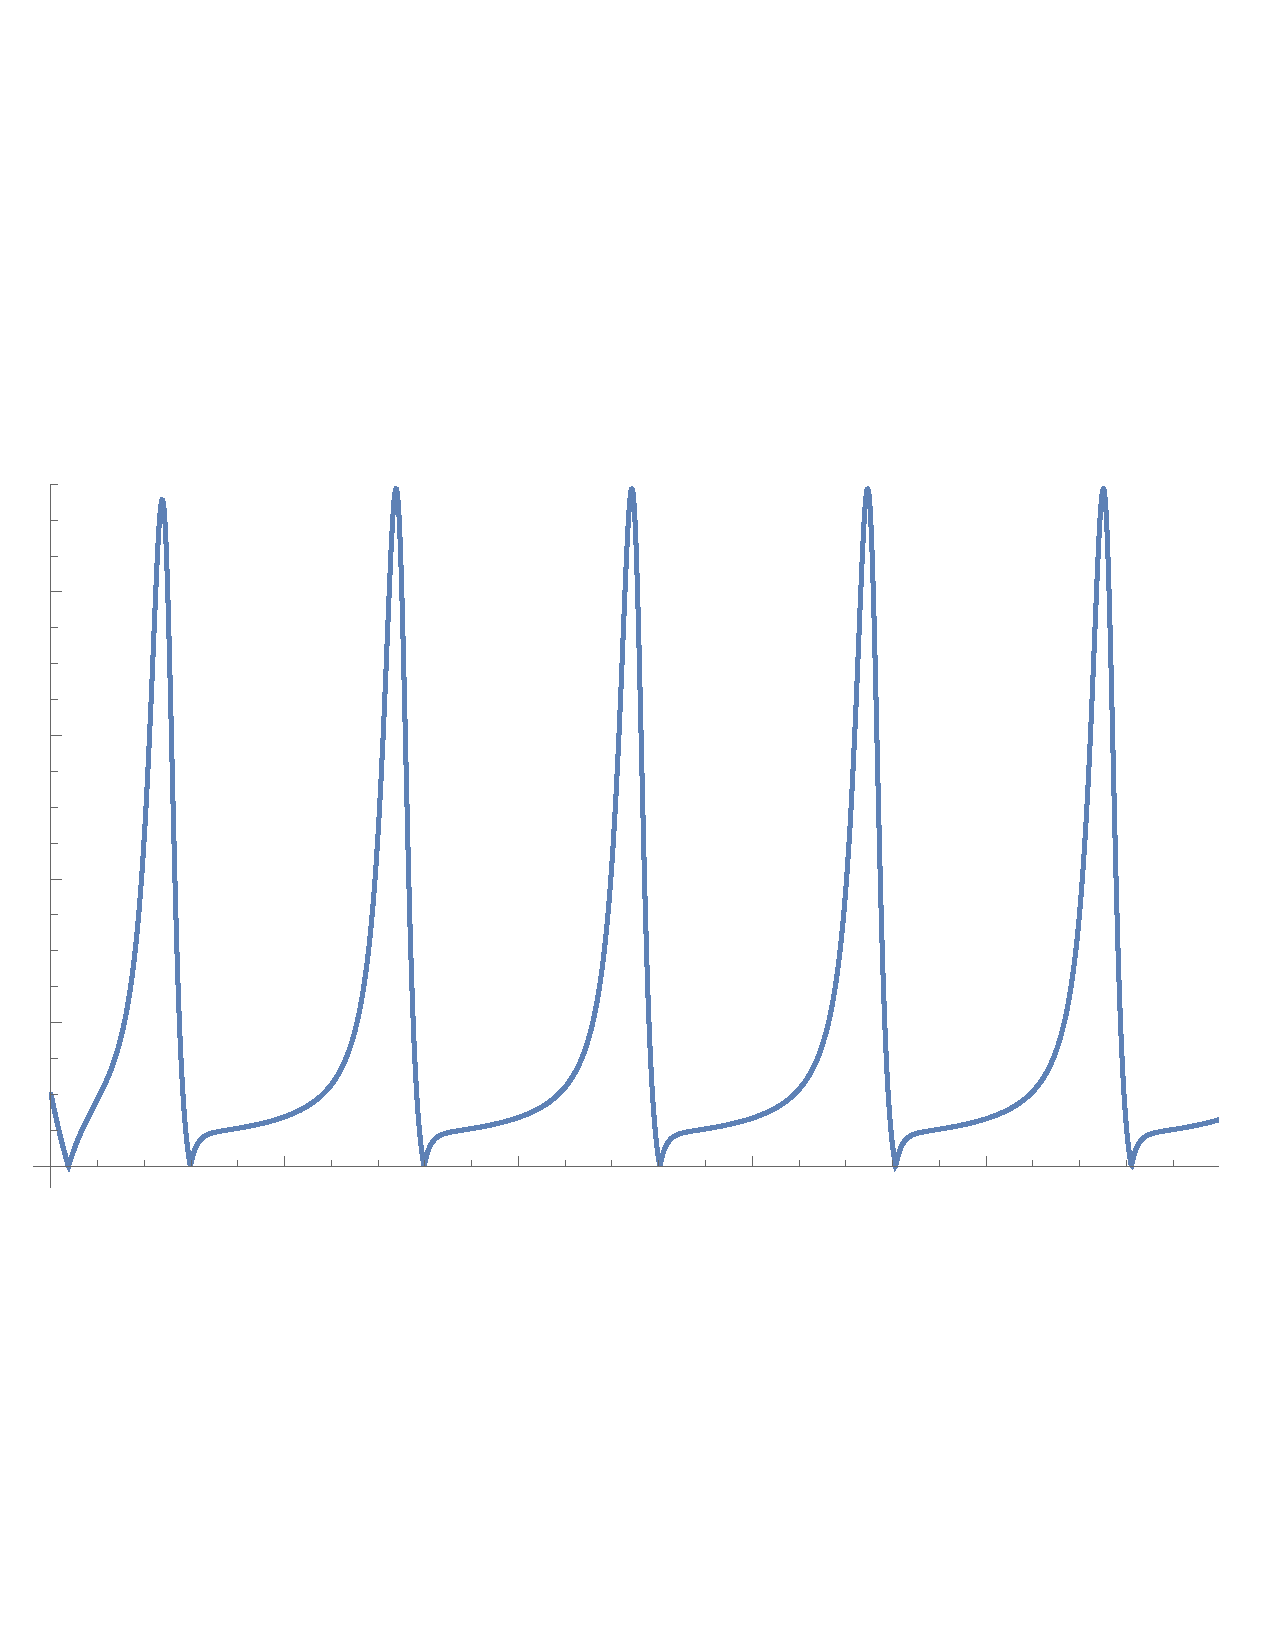
\includegraphics[width=.225\linewidth]{eq17_s.pdf}\\
\textbf{a:}{  $\gamma = 0 $}\hspace{30mm}\textbf{b:}{  $\gamma = 0.5 $}\hspace{30mm}\textbf{c:}{  $\gamma = 1 $}\hspace{30mm}\textbf{d:}{  $\gamma = 1.7 $}
\captionof{figure}{Plots of speed $\of{|\nu |}$ for varying values of $\gamma$. ({\bf a}) exhibits harmonic oscillations with high frequency,  ({\bf b}) a damped oscillator settling to a stable equilibrium point,  ({\bf c}) nearly immediate convergence to stability, and  ({\bf d}) relaxation oscillations of decreasing frequency as $\gamma\rightarrow\infty$ }
\end{center}
\end{posterbox}

%%%%%%%%%%%%%%%%%%%%%%%%%%%%%%

\begin{posterbox}[name=foottext, column=0, span=4, below=simulation, above = bottom, textborder=none,headerborder=none,boxheaderheight=0pt]{}
	\vspace{-4mm}
 	\hspace{-0.7cm}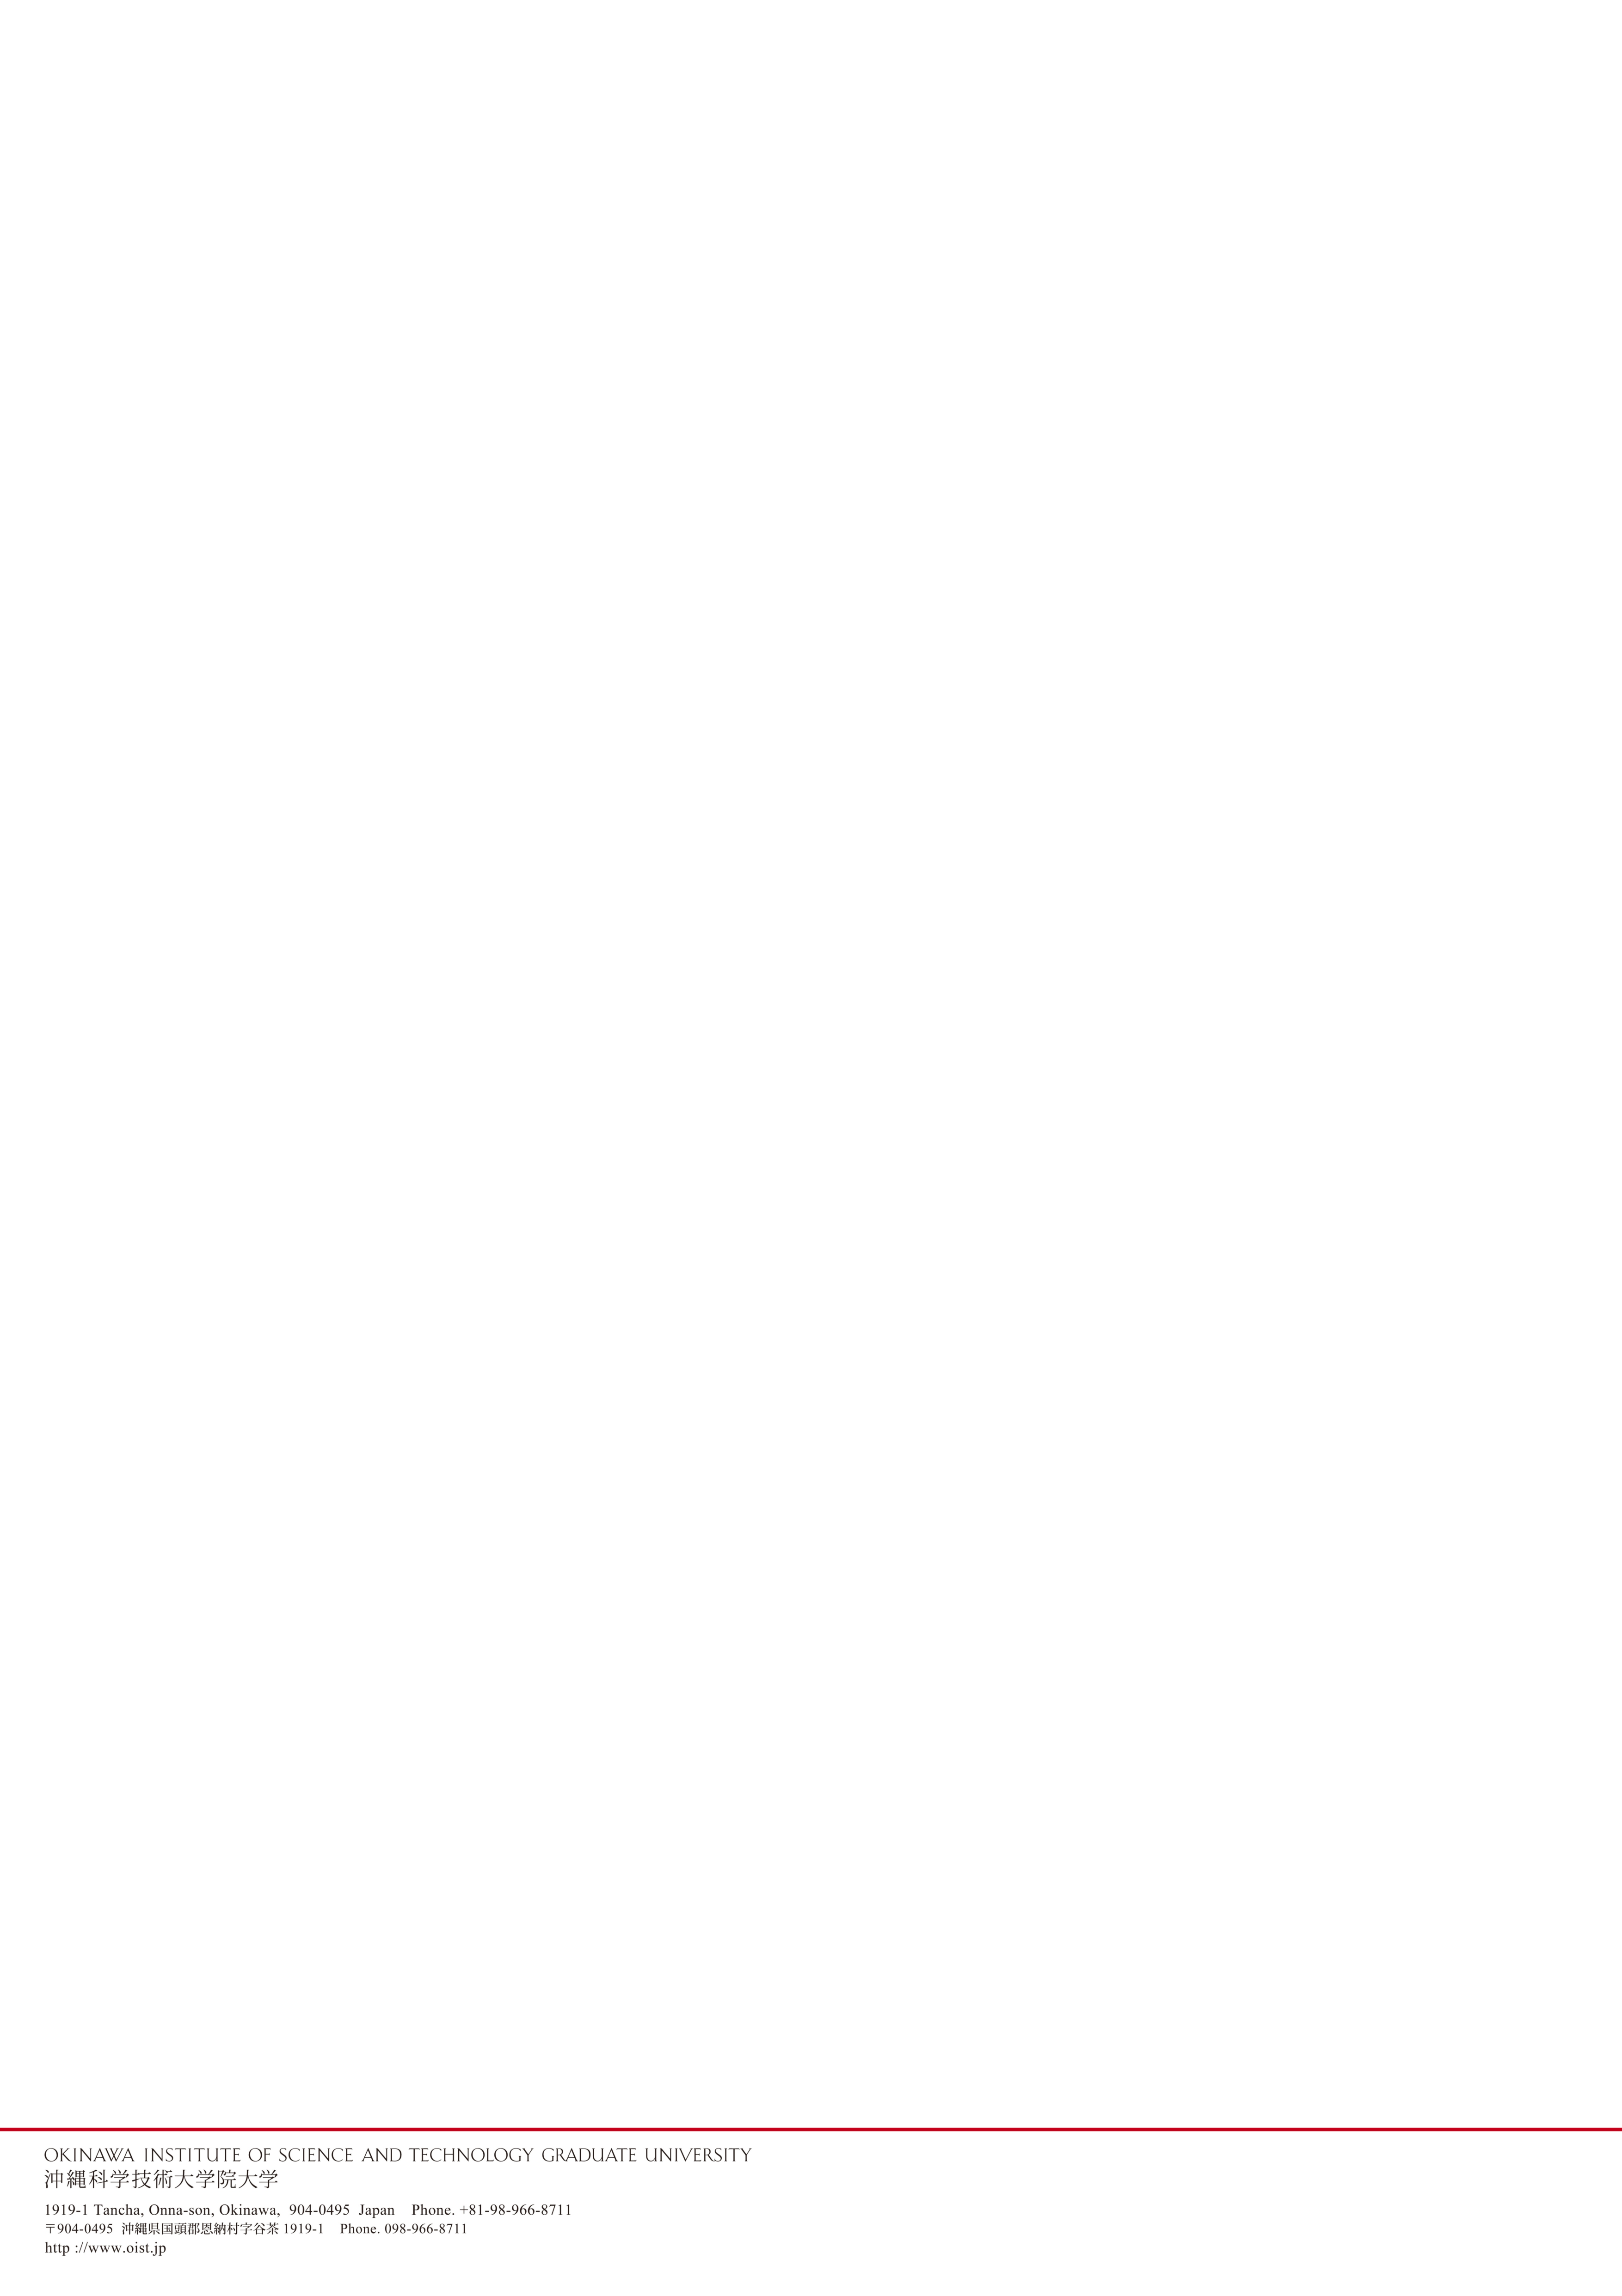
\includegraphics[width=1.2\linewidth]{A1_Vertical.pdf}
\end{posterbox}


\end{poster}
\end{document}